\documentclass[aspectratio=169,xcolor=dvipsnames]{beamer}
\usetheme{Berlin}

\usepackage[english]{babel}
\usepackage{hyperref}
\usepackage{graphicx}
\usepackage{booktabs}
\usepackage{amsmath}
\usepackage{lettrine}
\setbeamertemplate{caption}[numbered]
\usepackage[dvipsnames,svgnames,x11names]{xcolor}
\usepackage{xurl}
\usepackage{algorithm}
\usepackage{algorithmicx}
\usepackage{algpseudocode}
\usepackage{adjustbox}

% Configuración de enlaces y metadatos PDF
\hypersetup{
    colorlinks=true,
    linkcolor=cyan,
    filecolor=blue,
    urlcolor=blue,
    citecolor=blue,
}

%----------------------------------------------------------------------------------------
%	CODE LISTINGS SETTINGS
%----------------------------------------------------------------------------------------
\usepackage{listings}
\definecolor{backcolour}{rgb}{0.97,0.97,0.99}
\definecolor{codegreen}{rgb}{0,0.6,0}

\lstdefinestyle{MATLABStyle}{
  language=Matlab,
  basicstyle=\ttfamily\scriptsize,
  keywordstyle=\color{blue}\bfseries,
  commentstyle=\color{codegreen},
  stringstyle=\color{violet},
  breaklines=true,
  numbers=left,
  numbersep=5pt,
  frame=lines,
  backgroundcolor=\color{backcolour}
}
\lstset{style=MATLABStyle}

%----------------------------------------------------------------------------------------
%	INFORMACIÓN DEL TÍTULO
%----------------------------------

% Metadata
\title{Example 3: Simple Image Classification}
\subtitle{Using Deep Network Designer and CNNs}

\author{Prof. D.Sc. BARSEKH-ONJI Aboud}

\institute
{
    Facultad de Ingeniería \\
    Universidad Anáhuac México
}
\date{\today}

\AtBeginSection[]
{
  \begin{frame}{Agenda}
    \tableofcontents[currentsection]
  \end{frame}
}

\begin{document}

\begin{frame}
    \titlepage
\end{frame}

%------------------------------------------------
\section{Workflow Overview}
%------------------------------------------------

\begin{frame}{Workflow with Deep Network Designer}
    \begin{columns}
        \column{0.4\textwidth}
        Step-by-step process:
        \begin{enumerate}
            \item \textbf{Design:} Drag \& drop layers from the library.
            \item \textbf{Connect:} Link layers sequentially.
            \item \textbf{Analyze:} Verify dimension compatibility ($S, T, C, B$).
            \item \textbf{Export:} Generate code or export network object (\texttt{net\_1}) to workspace.
        \end{enumerate}
        
        \column{0.6\textwidth}
        \begin{figure}
            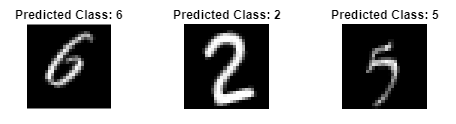
\includegraphics[width=\textwidth]{../Examples/Ex3/images/CreateImageClassificationNetworkUsingDeepNetworkDesignerExample_01.png}
            \caption{Deep Network Designer Interface.}
        \end{figure}
    \end{columns}
\end{frame}

%------------------------------------------------
\section{Network Architecture}
%------------------------------------------------

\begin{frame}{Input and Convolution Layers}
    \begin{columns}
        \column{0.5\textwidth}
        \textbf{1. Image Input Layer:}
        \begin{itemize}
            \item Size: $28 \times 28 \times 1$ (Grayscale).
            \item Normalization: Zero-center (default).
        \end{itemize}
        
        \textbf{2. Convolution 2D:}
        \begin{itemize}
            \item \textbf{32 Filters} of size $3 \times 3$.
            \item Feature extraction (edges, textures).
            \item Output depth becomes 32 chains.
        \end{itemize}
        
        \column{0.5\textwidth}
        \begin{figure}
            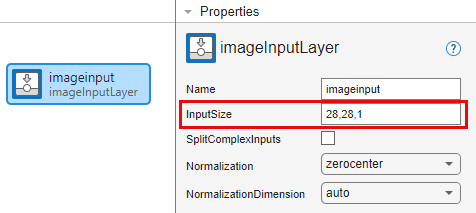
\includegraphics[width=0.9\textwidth]{../Examples/Ex3/images/CreateImageClassificationNetworkUsingDeepNetworkDesignerExample_02.png}
            \caption{Input and Feature Extraction layers.}
        \end{figure}
    \end{columns}
\end{frame}

\begin{frame}{Processing and Activation}
    \textbf{3. Batch Normalization:}
    \begin{itemize}
        \item Stabilizes training by normalizing layer inputs.
        \item Allows for higher learning rates.
    \end{itemize}
    
    \textbf{4. ReLU Layer:}
    \begin{itemize}
        \item Introduces non-linearity: $f(x) = \max(0, x)$.
        \item Essential for learning complex patterns.
    \end{itemize}
\end{frame}

\begin{frame}{Classification Head}
    \begin{columns}
        \column{0.6\textwidth}
        \textbf{5. Fully Connected Layer:}
        \begin{itemize}
            \item Output Size: \textbf{10} (Number of classes).
            \item Combines all local features for global decision.
        \end{itemize}
        
        \textbf{6. Softmax Layer:}
        \begin{itemize}
            \item Converts raw scores (logits) into probabilities summing to 1.
        \end{itemize}
        
        \textbf{7. Classification Layer:}
        \begin{itemize}
            \item Computes Cross-Entropy Loss during training.
        \end{itemize}
        
        \column{0.4\textwidth}
        \begin{figure}
            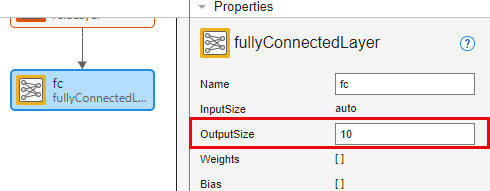
\includegraphics[width=0.8\textwidth]{../Examples/Ex3/images/CreateImageClassificationNetworkUsingDeepNetworkDesignerExample_03.png}
            \caption{Full Architecture.}
        \end{figure}
    \end{columns}
\end{frame}

%------------------------------------------------
\section{Understanding Dimensions (SSCB)}
%------------------------------------------------

\begin{frame}{Data Formats: S, T, C, B}
    MATLAB uses specific notation for tensors in the Network Analyzer.
    
    \begin{table}[]
        \centering
        \begin{tabular}{@{}cclp{5cm}@{}}
            \toprule
            \textbf{Tag} & \textbf{Name} & \textbf{Span.} & \textbf{Description} \\ \midrule
            \textbf{S} & Spatial & Espacial & Height and Width dimensions (e.g., $28 \times 28$). Reduced by pooling/convolution usually. \\
            \textbf{T} & Time & Tiempo & Temporal dimension. For static images, $T=1$. \\
            \textbf{C} & Channel & Canal & Depth/Feature Maps. Input=1 (Gray), Output Conv=32. \\
            \textbf{B} & Batch & Lote & Number of samples processed in parallel during training. \\ \bottomrule
        \end{tabular}
    \end{table}
\end{frame}

\begin{frame}{Analyzer View}
    \begin{figure}
        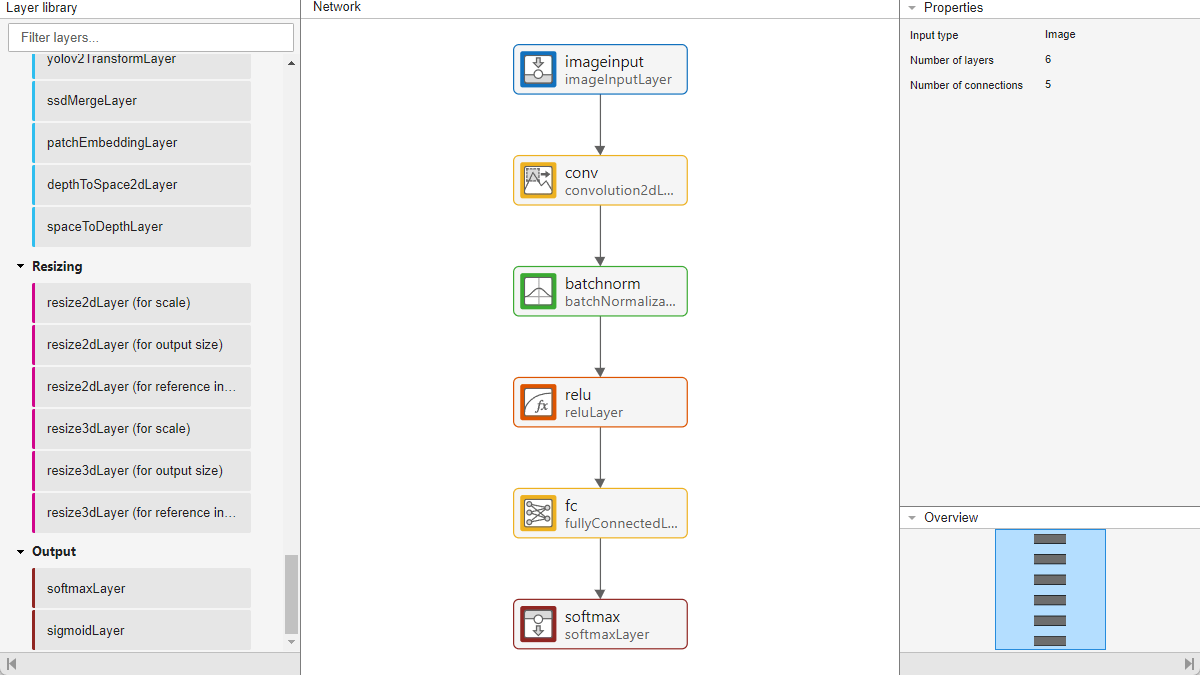
\includegraphics[width=0.7\textwidth]{../Examples/Ex3/images/CreateImageClassificationNetworkUsingDeepNetworkDesignerExample_04.png}
        \caption{Network Analyzer Table showing Activations in SSCB format.}
    \end{figure}
\end{frame}

%------------------------------------------------
\section{Training \& Results}
%------------------------------------------------

\begin{frame}{Training Progress}
    Training Config: \texttt{sgdm}, 4 Epochs, Accuracy Metric.
    
    \begin{figure}
        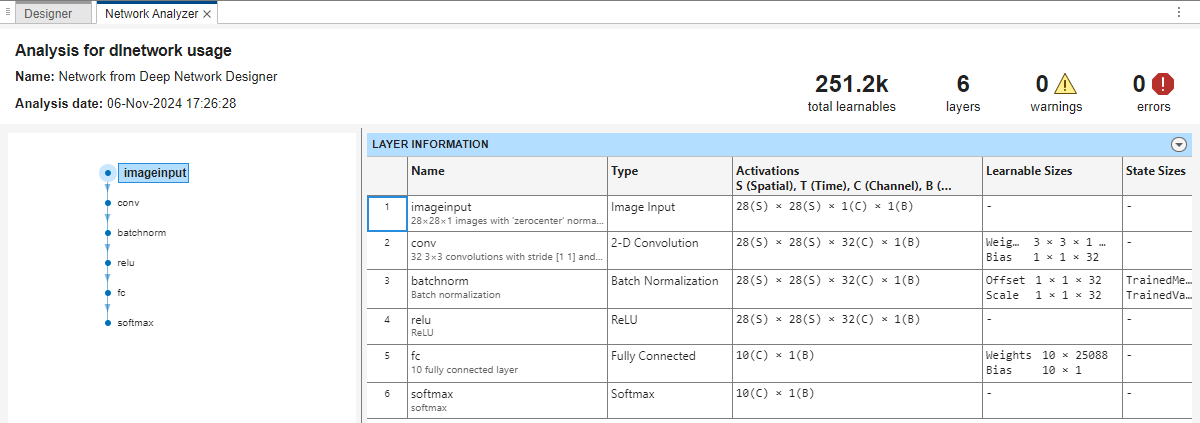
\includegraphics[width=0.65\textwidth]{../Examples/Ex3/images/CreateImageClassificationNetworkUsingDeepNetworkDesignerExample_05.png}
        \caption{Training Progress Plot (Accuracy vs. Iteration).}
    \end{figure}
\end{frame}

\begin{frame}[fragile]{Prediction Code}
    Using \texttt{testnet} or \texttt{minibatchpredict}:
    
\begin{lstlisting}[language=Matlab]
% Train the network
net = trainnet(imdsTrain, net_1, "crossentropy", options);

% Evaluate standard accuracy
accuracy = testnet(net, imdsValidation, "accuracy");

% Visualizing Predictions
scores = minibatchpredict(net, imdsValidation);
YPred = scores2label(scores, classNames);
\end{lstlisting}
\end{frame}

\begin{frame}{Validation Results}
    Example predictions on the validation set:
    
    \begin{figure}
        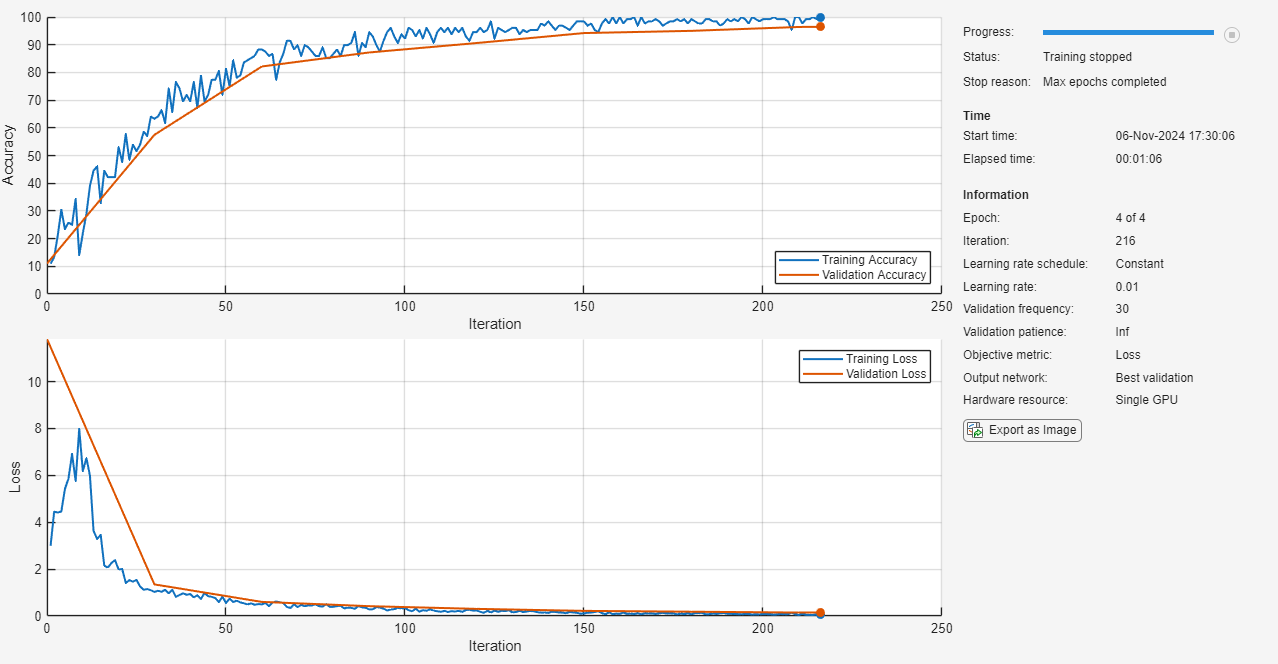
\includegraphics[width=0.5\textwidth]{../Examples/Ex3/images/CreateImageClassificationNetworkUsingDeepNetworkDesignerExample_06.png}
        \caption{Prediction Grid.}
    \end{figure}
\end{frame}



\end{document}
